\documentclass[a4paper]{article}
\usepackage{color}              %Farben, f.r \definecolor{}
\usepackage{amssymb}            %Mathematische Symbole
\usepackage{amsthm}             %Besseres \newtheorem
\usepackage{amsmath}           %Mathematische Umgebungen
\usepackage{mathtools}          %\xRightarrow, etc
\usepackage{mathrsfs}           %enthaelt \mathscr
\usepackage{graphicx}
\usepackage{enumerate}          % in-place numerations def.
\usepackage{fullpage}

\usepackage{array}
%\usepackage{multicol}
%\usepackage[notref,notcite]{showkeys}
%\usepackage{algorithm,algorithmic}
\usepackage{color}

\usepackage{graphicx}
\usepackage{xypic}
\entrymodifiers={+!!<0pt,\fontdimen22\textfont2>}
\usepackage[all]{xy}

\usepackage{float}
\usepackage{tikz}
\usepackage{tikz-cd}
\usepackage{tikz,fullpage}
\usetikzlibrary{arrows,%
                petri,%
                topaths}%
\usepackage{tkz-berge}
\usepackage[position=top]{subfig}
\usetikzlibrary{shapes.geometric}
\usetikzlibrary{decorations.markings}

\newtheoremstyle{myremark} % name
    {7pt}                    % Space above
    {7pt}                    % Space below
    {}  	                 % Body font
    {}                           % Indent amount
    {\bf}       	         % Theorem head font
    {.}                          % Punctuation after theorem head
    {.5em}                       % Space after theorem head
    {}  % Theorem head spec (can be left empty, meaning ‘normal’)

\theoremstyle{plain}
\newtheorem{lemma}{Lemma}
\newtheorem{theorem}[lemma]{Theorem}
\newtheorem{fact}[lemma]{Fact}
\newtheorem{definition}[lemma]{Definition}
\newtheorem{corollary}[lemma]{Corollary}
\newtheorem{proposition}[lemma]{Proposition}
\newtheorem{conjecture}[lemma]{Conjecture}
\newtheorem{observation}[lemma]{Observation}
\newtheorem{problem}[lemma]{Problem}
\newtheorem{notation}[lemma]{Notation}
\newtheorem*{claim}{Claim}

\theoremstyle{myremark}
\newtheorem{remark}[lemma]{Remark}
\newtheorem{example}[lemma]{Example}
\newtheorem{exercise}[lemma]{Exercise}
\newtheorem{algorithm}[lemma]{Algorithm}
\newtheorem{application}[lemma]{Application}
\newtheorem*{goal}{Goal}
\newtheorem*{summary}{Summary}
\newtheorem*{question}{Question}

%%%%%% EDIT HERE: %%%%%%%%%%%
\newcommand{\LECTURENUMBER}{0}
\newcommand{\LECTURETITLE}{Short title}
\newcommand{\LECTURESCRIBE}{Your name}

%% Dokument Beginn %%%%%%%%%%%%%%%%%%%%%%%%%%%%%%%%%%%%%%%%%%%%%%%%%%%%%%%%
\begin{document}
\thispagestyle{empty}

\begin{center}
	{\Large\bf Graph coloring}\\
	{\bf Lecture notes, vol. 8 \\ Chromatic polynomials, orientations, chromatic roots}\\
\end{center}
Lecturer: Michal Adamaszek \hfill Scribe: Giorgia L. G. Cassis
\begin{center}
\line(1,0){450}
\end{center}

%%%%%%% EDIT ALSO BELOW: %%%%%%%%%%%%%%%%

In the next pages, $G$ is always a graph, $V(G)$ its set of vertices and $E(G)$ its set of edges. 

\begin{lemma} Let $G,G_1,G_2$ be graphs such that $G=G_1 \cup G_2$ and $G_1 \cap G_2 \simeq K_k$ for some $k\geqslant 0$. Then
$$P_G(t)=\frac{1}{t^{\underline{k}}}P_{G_1}(t)P_{G_2}(t).$$
\begin{figure}[H]
\begin{center}
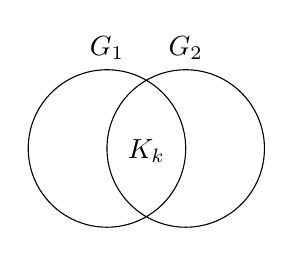
\begin{tikzpicture} 
\draw (-0.5,0) circle (1) (-0.5,1)  node [text=black,above] {$G_1$}
      (0.5,0) circle (1) (0.5,1)  node [text=black,above] {$G_2$};

\draw  (0, -0.3) node [text=black,above] {$K_k$};
\end{tikzpicture}
\end{center}
\end{figure}
\end{lemma}

\begin{proof}
Colour $G_1$ and colour $G_2$. Since $G_1 \cap G_2 \simeq K_k$, $G_1 \cap G_2$ uses $k$ different colours. It means that the colourings of $G_1$ and $G_2$ agree in $\frac{1}{P_{K_k}(t)}$ fraction of pairs.
\end{proof}

\begin{application}
\begin{enumerate}
\item $G=G_1 \sqcup G_2$ ($k=0$), then $$P_G(t)=P_{G_1}(t)P_{G_2}(t),$$
\item $v$ is a leaf in $G$ ($k=1$), then $$P_G(t)=\frac{1}{t}P_{K_2}(t)P_{G-v}(t)=\frac{1}{t}t(t-1)P_{G-v}(t)=(t-1)P_{G-v}(t),$$
\begin{figure}[H]
\begin{center}
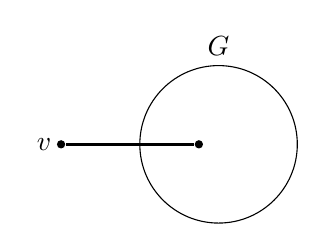
\begin{tikzpicture} 
\draw (0.5,0) circle (1) (0.5,1)  node [text=black,above] {$G$};

\draw  node[fill,circle,inner sep=0pt,minimum size=3pt] (n1) at (0.25,0) {} 
(0.25,0) node [text=black,above] {}
 
	node[fill,circle,inner sep=0pt,minimum size=3pt] (n2) at (-1.5,0) {}
(-1.5,0) node [text=black,left] {$v$};

\draw [line width = 1 pt, black, -] (n1) edge node {} (n2);
\end{tikzpicture}
\end{center}
\end{figure}
\item $G= K_2 \square P_n= C_4 \cup K_2 \square P_{n-1}$ ($k=2$), then $$P_G(t)=\frac{1}{t(t-1)}P_{C_4}(t)P_{K_2 \square P_{n-1}}(t),$$ and we can use this method recursively.
\begin{figure}[H]
\begin{center}
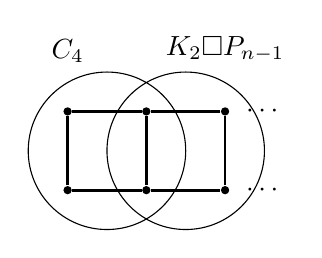
\begin{tikzpicture} 
\draw (-0.5,0) circle (1) (-1,1)  node [text=black,above] {$C_4$}
      (0.5,0) circle (1) (1,1)  node [text=black,above] {$K_2 \square P_{n-1}$};

\draw  node[fill,circle,inner sep=0pt,minimum size=3pt] (n1) at (-1,-0.5) {} 
(-1, -0.5) node [text=black,above] {}
 
	node[fill,circle,inner sep=0pt,minimum size=3pt] (n2) at (-1,0.5) {}
(-1,0.5) node [text=black,left] {}

node[fill,circle,inner sep=0pt,minimum size=3pt] (n3) at (0,-0.5) {} 
(0, -0.5) node [text=black,above] {}
 
	node[fill,circle,inner sep=0pt,minimum size=3pt] (n4) at (0,0.5) {}
(0,0.5) node [text=black,left] {}

node[fill,circle,inner sep=0pt,minimum size=3pt] (n5) at (1,-0.5) {} 
(1, -0.5) node [text=black,above] {}
 
	node[fill,circle,inner sep=0pt,minimum size=3pt] (n6) at (1,0.5) {}
(1,0.5) node [text=black,left] {}

(1.5,0.5) node (n7) [text=black] {$\cdots$}
(1.5,-0.5) node (n8) [text=black] {$\cdots$};

\draw [line width = 1 pt, black, -] (n1) edge node {} (n2)
[line width = 1 pt, black, -] (n3) edge node {} (n4)
[line width = 1 pt, black, -] (n5) edge node {} (n6)
[line width = 1 pt, black, -] (n1) edge node {} (n3)
[line width = 1 pt, black, -] (n3) edge node {} (n5)
[line width = 1 pt, black, -] (n2) edge node {} (n4)
[line width = 1 pt, black, -] (n6) edge node {} (n4);
\end{tikzpicture}
\end{center}
\end{figure}
\end{enumerate}
\end{application}

\begin{summary} $G$ is a graph with chromatic polynomial $P_G(t)$.
\begin{itemize}
\item $n=|V(G)|=deg(P_G)$,
\item $m=|E(G)|=-[t^{n-1}]P_G(t)$,
\item The number of connected components is $=max \{c: \ t^c \mid P_G(t) \}$,
\item $\chi(G) = 1+ max \{k: \ (t-k) \mid P_G(t) \}=1+ max \{k: \ t^{\underline{k}} \mid P_G(t) \}$,
\item The number of triangles is $={m \choose 2}-[t^{n-2}]P_G(t)$ (will be proved during the next exercise session),
\item The coefficients of the polynomial are integers with alternating signs.
\end{itemize}
\end{summary}

\begin{remark} It is hard to computer $P_G(t)$, otherwise we could easily compute $\chi(G)$. It is also hard to recognize chromatic polynomials.
\end{remark}

\begin{theorem} \emph{(June Huh, 2010)}
Suppose $G$ is connected with chromatic polynomial
$$P_G(t)=t^n-c_1t^{n-1}+c_2t^{n-2}-\cdots +(-1)^{n-1}c_{n-1}t.$$
Then the sequence $(1,c_1,c_2,\dots,c_{n-1})$ is log-concave, which means
$$c_{i-1}c_{i+1}\leqslant c_i^2 \quad \text{for all } i.$$
In particular, it is unimodal, which means
$$1 \leqslant c_1 \leqslant c_2 \leqslant \cdots \leqslant c_{k-1} \leqslant c_k \geqslant c_{k+1} \geqslant \cdots \geqslant c_{n-1}, \quad \text{for some } k.$$
\end{theorem}

\begin{proof}
This theorem proves a conjecture of Read from 1968. We will not prove the theorem (the proof involves algebraic geometry and singularity theory).
\end{proof}

\begin{exercise}
\begin{enumerate}
\item Why the name \textit{log-concave}?
\item Prove that a log-concave sequence of positive real numbers is unimodal.
\end{enumerate}
\end{exercise}

\begin{remark} We can prove $1 \leqslant c_1 \leqslant c_2 \leqslant \cdots \leqslant c_{\lfloor \frac{1}{2}(n-1)\rfloor}$.
\\ If $G$ is a tree, then
$$P_G(t)=t(t-1)^{n-1}=\sum_{i=0}^{n-1} {n-1 \choose i}(-1)^it^{n-i}\cdot t=t^n-{n-1 \choose 1}t^{n-1}+{n-1 \choose 2}t^{n-2}-\cdots.$$
The sequence $(1,c_1,c_2,\dots)$ is $(1,{n-1 \choose 1},{n-1 \choose 2},\cdots)$, and it is increasing up to the middle term.
\\ Now suppose that $G$ is connected, but not a tree. Then, by definition of a tree, there is an edge $e\in E(G)$ such that $G-e$ is still connected. For $i\leqslant \frac{1}{2}(n-1)$ we notice that
$$P_G(t)=P_{G-e}(t)-P_{G/e}(t) \Longrightarrow c_{i-1}(G)=c_{i-1}(G-e)-(-c_{i-2}(G/e))=c_{i-1}(G-e)+c_{i-2}(G/e).$$
We know $i\leqslant \frac{1}{2}(n-1)$ and $i-1 \leqslant \frac{1}{2}(n-2)=\frac{1}{2}(|V(G/e)|-1)$, hence by induction 
 $$c_{i-1}(G)\leqslant c_i(G-e)+c_{i-1}(G/e)=c_i(G)$$
which ends the induction step.
\end{remark}


\begin{question} What else does the chromatic polynomial count? And how?
\end{question}

\begin{definition} An \emph{orientation} of $G$ is a choice  of direction for every edge. This gives a directed graph. If $G$ has $m$ edges, then it has $2^m$ possible orientations (which might also be isomorphic).
\end{definition}

\begin{definition} An orientation is \emph{acyclic} if it has no closed directed walk. Let $a(G)$ be the number of acyclic orientations of $G$.
\end{definition}

\begin{theorem} \emph{(Stanley, 1973)}
If $G$ has $n$ vertices, then $a(G)=(-1)^nP_G(-1)$.
\end{theorem}

\begin{example}
\begin{itemize}
\item $G$ is a tree with $n$ vertices, then
$$a(G)=2^{n-1}=(-1)^n(-1)(-1-1)^{n-1}=(-1)^nP_G(-1),$$
\item $G$ is a cycle on $n$ vertices, then
\begin{align*}
a(G)&=2^n-2, \\
(-1)^nP_G(-1)&=(-1)^n[(-2)^n+(-1)^n(-2)]=(-1)^n[(-1)^n(2^n-2)]=a(G),
\end{align*}
\item $G=K_n$, then
\begin{align*}
(-1)^nP_G(-1)&=(-1)^n(-1)^{\underline{n}}=(-1)^n(-1)(-1-1)(-1-2)\cdots (-1-(n-1))=(-1)^n(-1)^nn!.
\end{align*}
An acyclic orientation is the same as ordering the vertices $v_1,v_2,\dots,v_n$ (there are $n!$ possibilities to do this) and then choosing the orientation
$$v_i\longrightarrow v_j, \quad \text{whenever } i>j.$$
\end{itemize}
\end{example}

\begin{proof}
Take $e=xy \in E(G)$. Write $a^+(G-e),a^-(G-e),a^0(G-e)$ for the number of acyclic orientations of $G-e$ such that:
\begin{itemize}
\item There is a directed walk in $G-e$ from $x$ to $y$ ($a^+$),
\item There is a directed walk in $G-e$ from $y$ to $x$ ($a^-$),
\item There is no directed walk either way ($a^0$).
\end{itemize}

\begin{claim} $a(G-e)=a^+(G-e)+a^-(G-e)+a^0(G-e)$. 
\end{claim}
\begin{proof}
An acyclic orientation in $G-e$ cannot have directed walks $x\longrightarrow y$ and $y\longrightarrow x$ at the same time. These three sets are therefore disjoint and they give all the possibilities.
\end{proof}

\begin{claim} $a(G/e)=a^0(G-e)$. 
\end{claim}
\begin{proof}
Take an orientation of $G-e$ with no walk $x\longrightarrow y$ or $y\longrightarrow x$. For any $z\in N_{G-e}(x)\cap N_{G-e}(y)$, the edges $xz$ and $yz$ have the same orientation (if not, there would be a walk $x\longrightarrow z\longrightarrow y$ or $y\longrightarrow z\longrightarrow x$), hence either  
$$x\longrightarrow z \text{ and } y\longrightarrow z$$
or
$$z\longrightarrow x \text{ and } z\longrightarrow y.$$
The orientation of $G-e$ determines then an orientation of $G/e$ (the edges $xz$ and $yz$ are compatible under the contraction). This orientation is also acyclic (a directed walk from $xy$ to itself would imply a directed walk in $G-e$ from $x$ or $y$ to $y$ or $x$). This also works vice versa.
\\ The idea here was that 
$$\text{Closed walks in } G/e = \text{Walks } x\longrightarrow y \text{ or } y\longrightarrow x \text { in } G-e.$$
\end{proof}

\begin{claim} 
$a(G)=a^+(G-e)+a^-(G-e)+2a^0(G-e)$. 
\end{claim}
\begin{proof}
For the first two terms there is only one way to extend the orientation of $G-e$ without closing a cycle in $G$. In the last case the edge $xy$ can be oriented both ways, since we don't have a walk from $x$ to $y$ or from $y$ to $x$.
\end{proof}

By these three claims we obtain
\begin{align*}
a(G)&=a^+(G-e)+a^-(G-e)+2a^0(G-e)= \\
&= a^+(G-e)+a^-(G-e)+a^0(G-e)+a^0(G-e)= \\
&= a(G-e)+a^0(G-e)= \\
&= a(G-e)+a(G/e)
\end{align*}
We complete the proof by using induction:
\begin{itemize}
\item $G=K_1$, then $a(G)=1=(-1)^1P_{K_1}(-1)$,
\item Pick an edge $e\in E(G)$, then (by induction assumption)
\begin{align*}
a(G)&=a(G-e)+a(G/e)= \\
&= (-1)^nP_{G-e}(-1)+(-1)^{n-1}P_{G/e}(-1)= \\
&= (-1)^n[P_{G-e}(-1)-P_{G/e}(-1)]= \\
&= (-1)^nP_G(-1)
\end{align*}
\end{itemize}
\end{proof}

\begin{definition} $\alpha \in \mathbb{C}$ is a \emph{chromatic root} if $P_G(\alpha)=0$ for some graph $G$.
\end{definition}

\begin{observation}
\begin{enumerate}
\item Every natural number is a chromatic root,
\item For any $G$ different from the empty graph, $P_G(0)=0$,
\item For any $G$ with at least one edge, $P_G(1)=0$,
\item If $\alpha$ is a chromatic root, then so is $\alpha+1$,
\begin{proof}
We proved in the exercise session that $P_{G+K_1}(\alpha+1)=(\alpha+1)P_G(\alpha)$,
\end{proof}
\item The set of chromatic roots is countable (it is a subset of the algebraic numbers).
\end{enumerate}
\end{observation}



\begin{proposition} There is no chromatic root in $(- \infty, 0)\cup (0,1)$.
\end{proposition}

\begin{proof}
$\alpha <0$ is not a root of $P_G(t)$, since the coefficients of the polynomial have alternating signs.
\\
\\ Take $\alpha \in (0,1)$. Because $P_{G\sqcup H}(t)=P_G(t)P_H(t)$, it suffices to prove that $P_G(\alpha)\neq 0$ for any connected graph. Apply the deletion-contraction rule to $G$, in such a way that all the intermediate graphs are connected. At each step, either $G$ is a tree (and we stop splitting) or there is an edge $e\in E(G)$ such that $G-e$ is still connected.
\\
\\ A branch of this splitting process with $i$ contractions
\begin{itemize}
\item ends with an $(n-i)$-vertex tree,
\item introduces a sign of $(-1)^i$,
\item contributes $t(t-1)^{n-i-1}$ to $P_G(t)$.
\end{itemize}
Define $d_i$ as the number of branches ending with an $(n-i)$-vertex tree, then
$$P_G(t)=\sum d_i(-1)^it(t-1)^{n-i-1},$$
and of course we have $d_i\geqslant 0$.
Evaluate $P_G(\alpha)$ for $\alpha \in (0,1)$:
$$sgn\{d_i(-1)^i\alpha (\alpha-1)^{n-i-1} \}=(-1)^i\cdot 1\cdot (-1)^{n-i-1}=(-1)^{n-1},$$
which means that all monomials in $P_G(\alpha)$  evaluate to positive or all evaluate to negative, hence $P_G(\alpha) \neq 0$ as $d_i>0$ for at least one $i$. 
\end{proof}

\begin{remark} We used the deletion-contraction principle, but only until we reached trees (since we already know their chromatic polynomial).
\end{remark}


\begin{theorem} \emph{(Jackson, Thomassen)}
There are no chromatic roots in $(- \infty, 0)\cup (0,1)\cup (1,\frac{32}{27}).$ Moreover, the constant $\frac{32}{27}$ is optimal. 
\end{theorem}

\begin{theorem} \emph{(Sokal)}
The chromatic roots are dense in $\mathbb{C}$.
\end{theorem}

\begin{theorem} \emph{(Birkhoff, Lewis)}
If $G$ is planar, then $P_G(t)>0$ for all $t\in [5,\infty)$.
\end{theorem}

\begin{remark} Moreover, it is conjectured that if $G$ is planar, then $P_G(t)>0$ for all $t\in [4,\infty)$.
\end{remark}
\end{document}




